\documentclass{bredelebeamer}
\usepackage{subfig}

%%%%%%%%%%%%%%%%%%%%%%%%%%%%%%%%%%%%%%%%%%%%%%%%
\title[Kubernetes]{Kubernetes}
% Titre du diaporama

\subtitle{manage application, not machines}
% Sous-titre optionnel

\author{N. Salleron B. Affes}
% La commande \inst{...} Permet d'afficher l' affiliation de l'intervenant.
% Si il y a plusieurs intervenants: Marcel Dupont\inst{1}, Roger Durand\inst{2}
% Il suffit alors d'ajouter un autre institut sur le modéle ci-dessous.

\date{Lundi 12 Février 2018}
% Optionnel. La date, généralement celle du jour de la conférence

\subject{NMV}
% C'est utilisé dans les métadonnes du PDF

\logo{

\includegraphics[scale=0.03]{images/logo.jpg}
}

%%%%%%%%%%%%%%%%%%%%%%%%%%%%%%%%%%%%%%%%%%%%%%%%%%%%%%%%%%%%%%%%%%%%%
\begin{document}

\begin{frame}
  \titlepage
\end{frame}

\begin{frame}{Sommaire}
  \tableofcontents
  % possibilité d'ajouter l'option [pausesections]
\end{frame}

\section{Introduction}
\subsection{Introduction}

\begin{frame}{Historique}
\begin{block}{Une longue émergence}
\begin{itemize}
\item Borg
	\begin{itemize}
	\item Démarrage en 2004.
	\item Développé en interne.
	\item Manager de containers.
	\item Objectif : réduction des coups en partageant machines et applications.
	\item \textbf{Inconvéniant : notion de travail, gestion des ports}
	\item \textbf{Non open-source.}
	\end{itemize}	\pause
\item Omega	
	\begin{itemize}
	\item Fils de Borg.
	\item Amélioration de l'écosystème apporté par Borg.
	\item  \textbf{Non open-source.}
	\end{itemize}   \pause
\item Kubernetes
	\begin{itemize}
	\item Adaptable à plusieurs infrastructure cloud.
	\item  \textbf{Open-source.}
	\end{itemize}
\end{itemize}
\end{block}
\end{frame}

\begin{frame}{Introduction}
%Texte normal \alert{Texte Alert}  \exemple{Texte exemple} \emph{Texte emphase}
\begin{columns}
\begin{column}{0.5\textwidth}

Nom venant du Grec, crée par 3 ingénieurs de chez Google en 2014.
\begin{itemize}
\item \textit{Orchestrateur} - Gestionnaire de conteneur.
\item Exécute et manages des containers.
\item Propose une API permettant la gestion de plusieurs clouds (Google, Microsoft, Amazon, et pleins d'autres).
\item 100\% Open Source écrit en Go.
\end{itemize}


\end{column}
\begin{column}{0.5\textwidth}


\begin{figure}
\centering
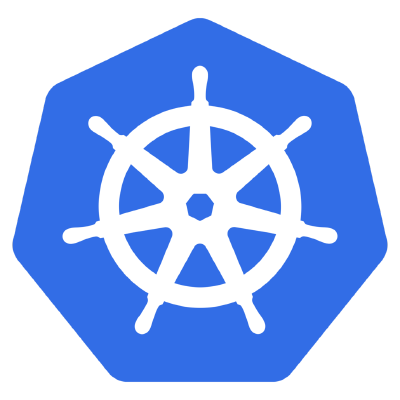
\includegraphics[scale=0.15]{images/img1.png}
\caption{Logo de Kubernetes}
\end{figure}

\end{column}
\end{columns}

\vspace{10px}
Il permet de se focus sur les applications et non sur le déploiement.  
Google exécute 2 milliards de conteneurs par semaine avec ces systèmes.\\\pause
\vspace{10px}
Dernière version : 1.9.3 (sortie il y a 3 jours) \\ \pause

\vspace{10px}
\begin{center}
\textit{"manage application, not machines" - Tim Hockin}
\end{center}

\end{frame}

\begin{frame}{Popularité}
Évolution des recherches entre \textcolor{Framableu}{Kubernetes}, \textcolor{Framarouge}{Mesos}, \textcolor{Framajaune}{Docker Swarm}
\begin{center}
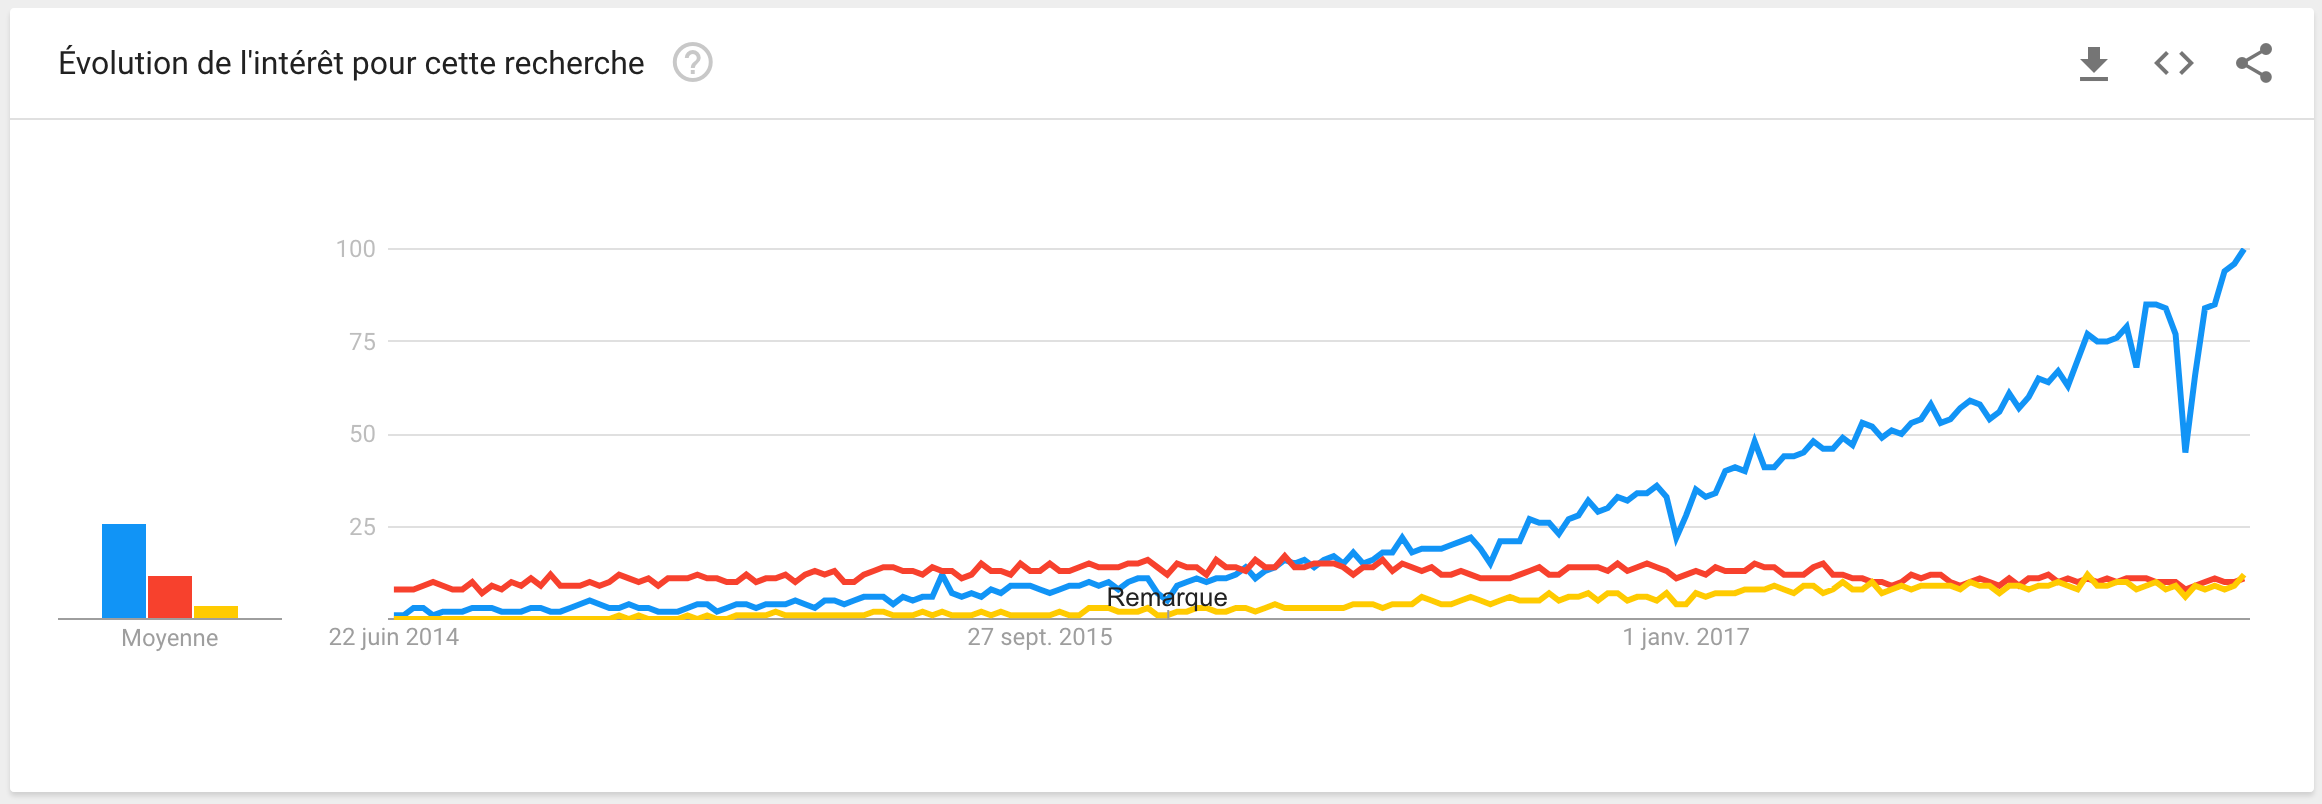
\includegraphics[scale=0.25]{images/img2.png}
\end{center}\pause
Une communauté très active : 
\begin{itemize}
\item Actuellement 61000 commits avec plus de 1500 contributeurs
\end{itemize}
\begin{center}
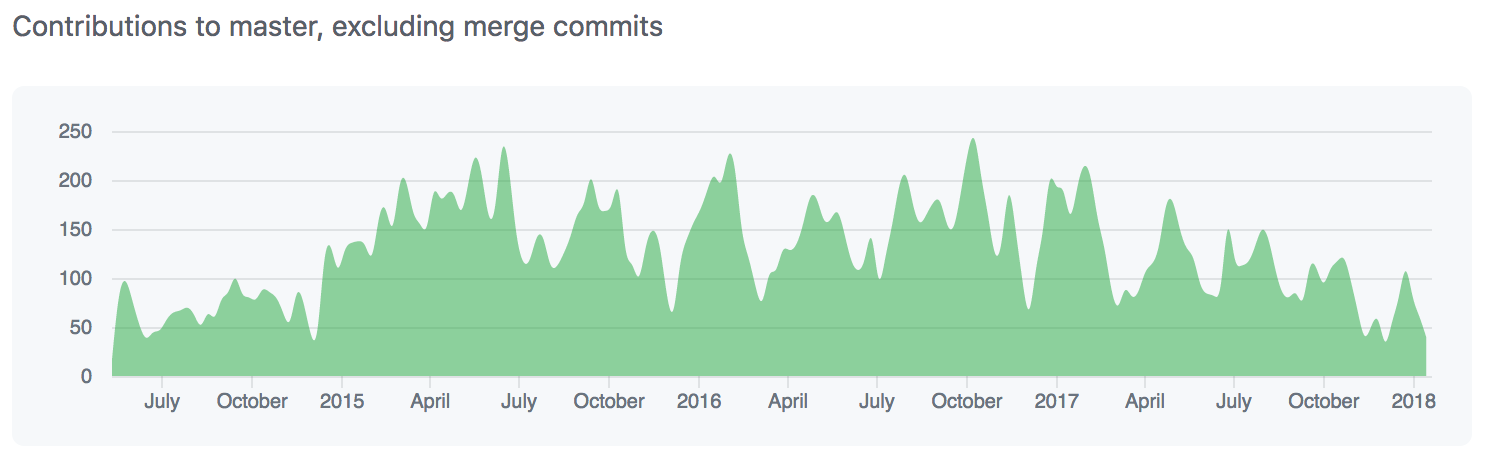
\includegraphics[scale=0.3]{images/img3.png}
\end{center}
\end{frame}

\section{Docker}
\subsection{Some few things about Docker}
\begin{frame}
\begin{center}

\includegraphics[scale=0.3]{images/img5.png}
\end{center}
\end{frame}
\begin{frame}
Docker est un conteneur léger, permettant de l'isolation entre les processus.
\begin{center}
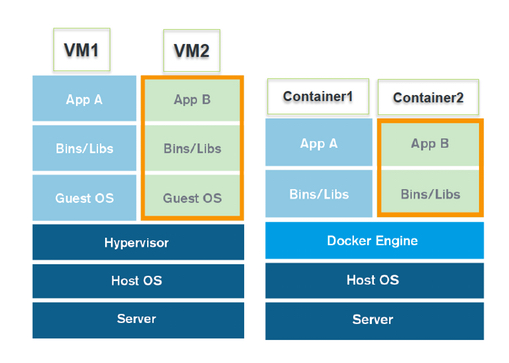
\includegraphics[scale=0.3]{images/img4.jpg}
\end{center}
\begin{itemize}
\item Retire le coût de la virtualisation (pas de gestion hardware)
\item Retire le coût d'exécution de plusieurs OS.
\end{itemize}

\end{frame}

\begin{frame}
Docker se base sur deux technologies du noyau : 
\begin{itemize}
\item CGroups
\item Namespace
\end{itemize} \pause

\begin{exampleblock}{Control Groups}
Feature kernel qui permet de contrôler, limité et isoler l'usage des ressources pour un processus ou une collection de processus. 
\end{exampleblock} \pause


\begin{block} {CGroups Isolation}
\begin{itemize}
\item  Quantitative Isolation : Les CGroups ne peuvent pas avoir plus de pages que la limite imposé.
\item Qualitative Isolation : Les CGroups doivent accéder à leur mémoire comme si elles étaient seules sur la machine.
\end{itemize}
\end{block} \pause

\begin{exampleblock}{Namespace}
Feature linux qui permet de créer une vue local pour les ressources d'un systèmes. Les ressources en dehors du namespace ne sont pas visible. 
\end{exampleblock}
\end{frame}


\section{Kubernetes  Core Concept}
\subsection{Pods}

\begin{frame}{Kubernetes}
\begin{center}

\includegraphics[scale=0.3]{images/img6.png}
\end{center}
\end{frame}

\begin{frame}{Pods}

\begin{columns}
\begin{column}{0.5\textwidth}
\begin{figure}
\centering
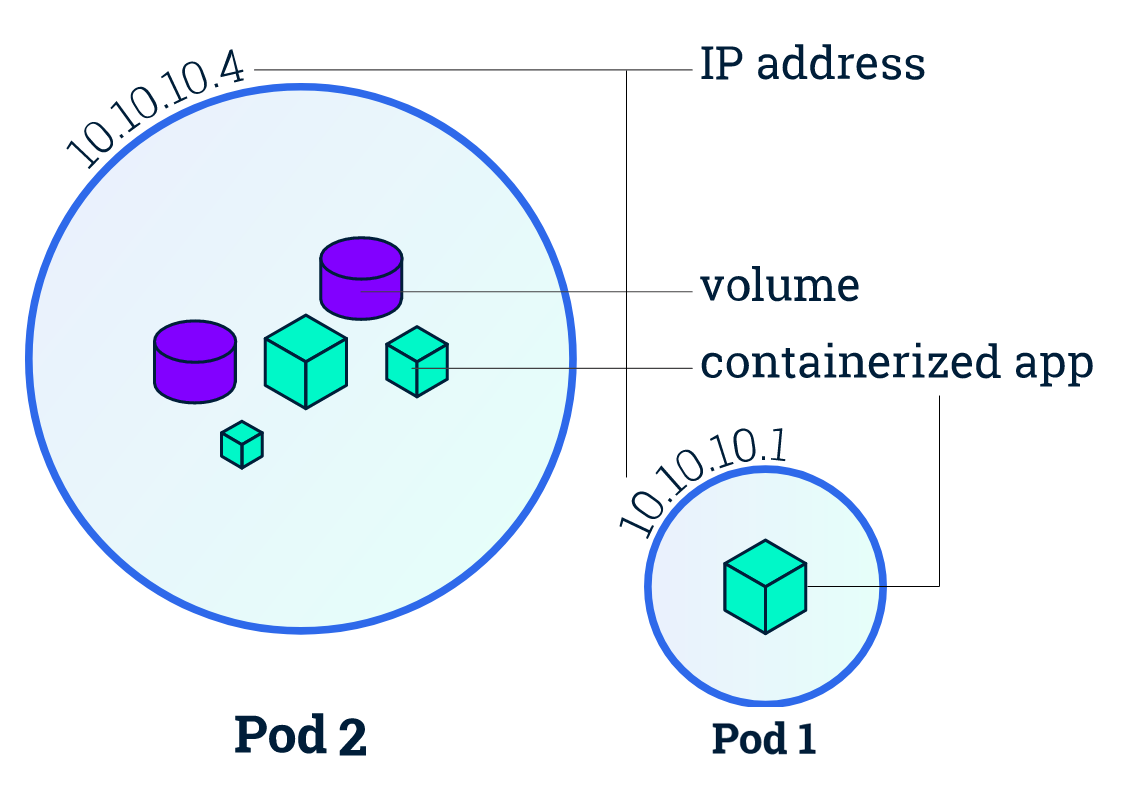
\includegraphics[scale=0.25]{images/img7.png}
\caption{Les Pod dans Kubernetes}
\end{figure}
\end{column}
\begin{column}{0.5\textwidth}
\begin{block}{Caractéristiques du Pod}

\begin{itemize}
\item Unité de base de l'ordonnancement. 											\pause
\item Vue abstraite de composants conteneurisés.								\pause
\item Il peut regrouper 1 ou * conteneurs. \\=> Couplage fort.				\pause
\item Chaque pod possède une adresse IP unique (limité au cluster).		\pause
\item Un Pod peut définir un volume. 
		%comme un répertoire sur un disque local ou réseau.
		Il a la même durée de vie que le Pod.
\end{itemize}
\end{block}																							\pause
\end{column}



\end{columns}
\vspace{4px}
Bénéfices du pod : 
\begin{itemize}
\item Plusieurs conteneurs dans 1 Pod\\
=> Processus qui ont besoin d'interroger un autre processus avec une faible latence.		\pause
\item Utilisable sous plusieurs environnements (fichier de configuration indépendant de la plateforme)		\pause
\item Mortel : un container peut mourir.		
\end{itemize}
\end{frame}

\subsection{Label et Selector}

%Kubernetes permet à des clients (utilisateurs et composants internes) d'attacher des paires clés-valeurs appelées "labels" à n'importe quel objet d'API dans le système, par exemple les pods et les nodes. Par correspondance, les "label selectors" sont des interrogations faites sur les labels en lien avec des objets15.

%Labels et selectors constituent le premier mécanisme de groupement dans Kubernetes, et sont utilisés pour déterminer les composants sur lesquels appliquer une opération18.

%Par exemple, si les Pods d'une application ont des labels pour un système tier ("front-end", "back-end", par exemple) et une release_track ("preproduction", "production", par exemple), alors une opération sur tous les nodes "back-end" et "preproduction" peuvent utiliser un label selector comme suit19 :

%    tier=back-end AND release_track=preproduction

\begin{frame}{Label et Selector}
\begin{columns}
\begin{column}{0.5\textwidth}
\begin{block}{Label}
\begin{itemize}
\item Méta-données arbitraire attaché à un objet.
\item Forme (K:V)
\item Représente généralement une identité.
\end{itemize}
\end{block}
\begin{block}{Selector}
\begin{itemize}
\item Permet de sélectionner plusieurs objets.
\item API supporte deux types de selector : 
\begin{itemize}
\item equality-based : "==", "=", "!=" %Question
\item set-based : "in", "notin", "exists"
\end{itemize}
\end{itemize}
\end{block}
\end{column}
\begin{column}{0.5\textwidth}
\begin{figure}
\centering
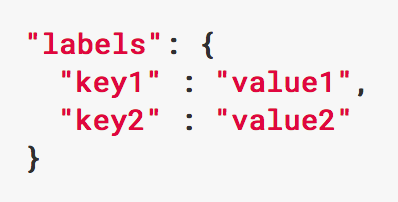
\includegraphics[scale=0.4]{images/img9.png}
\caption{Exemple K:V format JSON}
\end{figure}
\begin{figure}
\centering
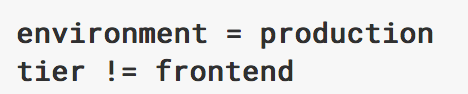
\includegraphics[scale=0.4]{images/img11.png}
\caption{Selector \textit{"equality-based"}}
\end{figure}
\begin{figure}
\centering
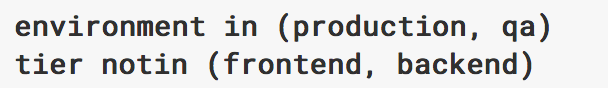
\includegraphics[scale=0.4]{images/img10.png}
\caption{Selector \textit{"set-based"}}
\end{figure}
\end{column}
\end{columns}
\end{frame}

\begin{frame}{Exemple d'utilisation}
\begin{figure}
\centering
\includegraphics<1>[scale=0.6]{images/img12.png}
\includegraphics<2>[scale=0.5]{images/img13.png}
\includegraphics<3>[scale=0.5]{images/img14.png}
\includegraphics<4>[scale=0.5]{images/img15.png}
\includegraphics<5>[scale=0.5]{images/img16.png}
\caption{Exemple avec différents selectors}
\end{figure}
\end{frame}


\subsection{Réplication et Mise à jour continue}
\begin{frame}{Les ReplicatSet}
\begin{columns}
\begin{column}{0.5\textwidth}

\begin{block}{Objectifs}
\begin{itemize}
	\item Gère l'unité basique dans Kubernete, le Pod.
	\item Il s'assure que le nombre de Pod voulu est présent.
	\begin{itemize}
		\item Groupe les Pods via des Selectors
		\item Si n < LIMIT : start Pod
		\item Si n > LIMIT : kill Pod
	\end{itemize}
	\item Les Pods répliqués n'ont pas d'identité propre.
	\item Ce sont des consommables.
	\item Peut-être utilisé pour une mise à l'échelle horizontale automatisé.
\end{itemize}
\end{block}
\end{column}
\begin{column}{0.5\textwidth}

\begin{figure}
\centering
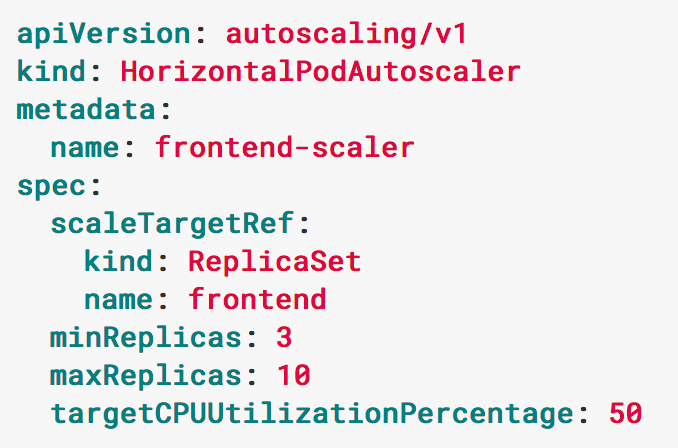
\includegraphics[scale=0.4]{images/img17.png}
\caption{Mise à l'échelle horizontale automatique}
\end{figure}
\end{column}
\end{columns}

\begin{alertblock}{Attention}
Les ReplicatSet sont déconseiller pour faire de la mise à jour continue. \\
=> A utiliser seulement pour des applications n'ayant pas besoin de mise à jour
\end{alertblock}
\end{frame}

\subsection{Deployment et Service}
\begin{frame}{Deployment et Service}
\begin{columns}
\begin{column}{0.6\textwidth}
\begin{block}{Deployment}
\begin{itemize}
	\item Possède et gère 1 ou plusieurs Replica Sets.
	\item Permet la mise à jour continue avec 3 paramètres: 
	\begin{itemize}
	\item minReadySeconds %: Bootup Time de l'application\\
	%\vspace{2px}
	%=> Par default kubernetes considère que l'application est disponible quand Pod disponible.
	\item maxSurge %: Indique le nombre de pod supplémentaire pendant le processus d'exécution.
	\item maxUnavailable% : Nombre de pod pouvant être indisponible pendant le processus de mise à jour.
	\end{itemize}
	\item Permet également le rollback après deployment.
\end{itemize}
\end{block}
\begin{exampleblock}{Service}
\begin{itemize}
\item Une abstraction d'un ensemble logique de pod et d'une politique d'accès aux Pods.
\item Adapté aux micro-services
\item Load-balancing
\end{itemize}
\end{exampleblock}
\end{column}
\begin{column}{0.4\textwidth}
\begin{figure}
\centering
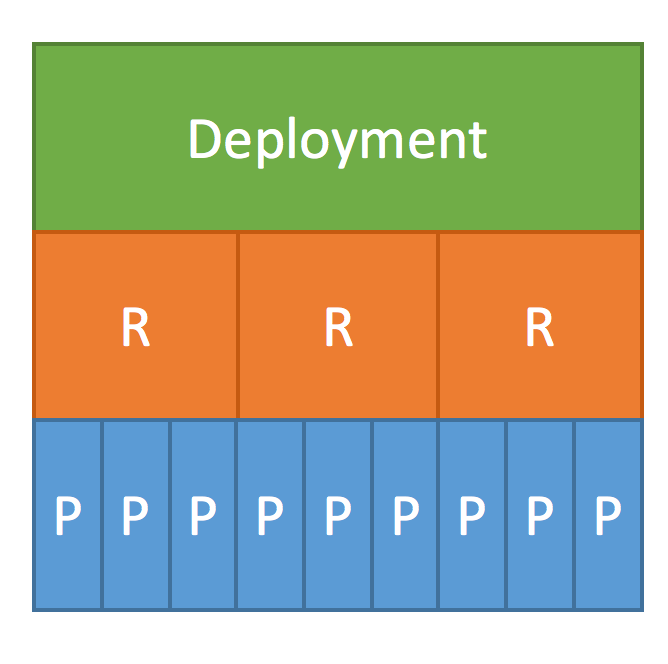
\includegraphics[scale=0.4]{images/img18.png}
\caption{Relation entre Objet Deployment, ReplicatSet et Pod}
\end{figure}

\end{column}
\end{columns}
\end{frame}
\begin{frame}{Exemple du Rolling-Update}
\begin{figure}
\centering
\includegraphics<1>[scale=0.25]{images/img19.png}
\includegraphics<2>[scale=0.25]{images/img20.png}
\includegraphics<3>[scale=0.25]{images/img21.png}
\includegraphics<4>[scale=0.25]{images/img22.png}
\caption{Exemple du Rolling Update tiré de la documentation Kubernetes}
\end{figure}
\end{frame}

\section{Kubernetes Architecture Concept}
\subsection{Architecture concept}

\subsection{Kubernetes Node}
\begin{frame}{Kubernetes Node i.e Worker Node}
\begin{columns}
\begin{column}{0.3\textwidth}

\begin{figure}
\centering
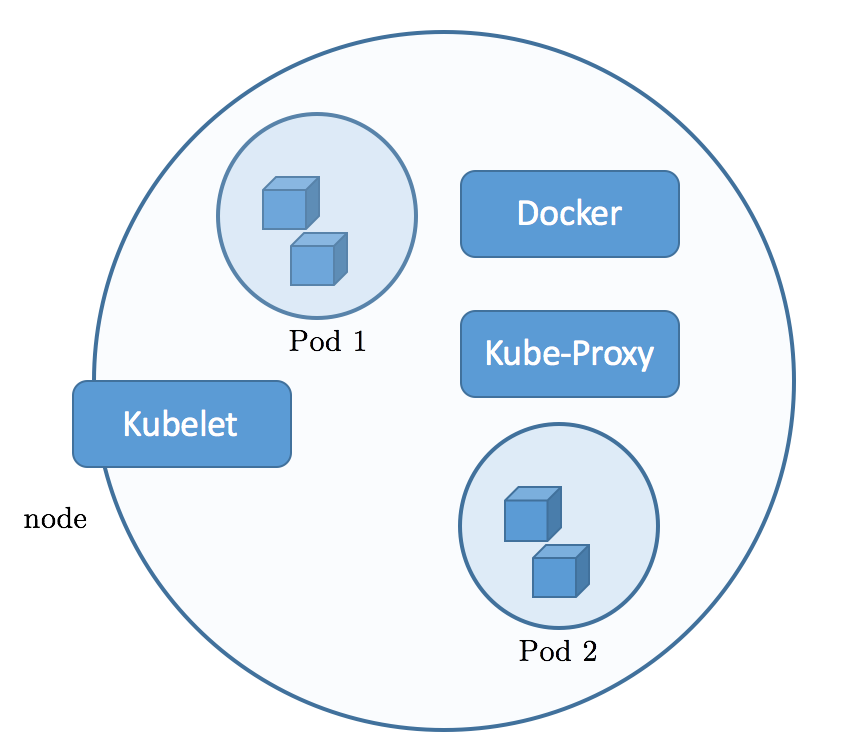
\includegraphics[scale=0.2]{images/img23.png}
\caption{Exemple de node}
\end{figure}


\end{column}
\begin{column}{0.7\textwidth}
\begin{block}{Rôle du node}
\begin{itemize}
\item Les pods sont exécuté dans des nodes. 
\item Il contient les services de gestion et de communications entre les containers.
\item Il assigne les ressources au containers qui sont ordonnancé par le master node.
\end{itemize}
\end{block}\pause
\end{column}
\end{columns}
\begin{block}{Kubelet}
\begin{itemize}
\item Il est responsable de l'exécution (start/stop/maintenance)
\item Il surveille l'état d'un pod, % et s'il n'est pas dans l'état voulu, le pod sera redéployé sur le même node. 
communique l'état du node au master node.
\item Interaction avec un moteur Docker sous-jacent pour démarrer des conteneurs.
\end{itemize}
\end{block}\pause
\begin{block}{Kube-proxy}
\begin{itemize}
\item Routage du trafic vers le conteneur grâce à l'IP/Port et \textit{répartiteur de charge}.
\end{itemize}
\end{block}
\end{frame}

\subsection{Kubernetes Master}
\begin{frame}{Kubernetes Master}
\begin{columns}
\begin{column}{0.4\textwidth}
\begin{figure}
\centering
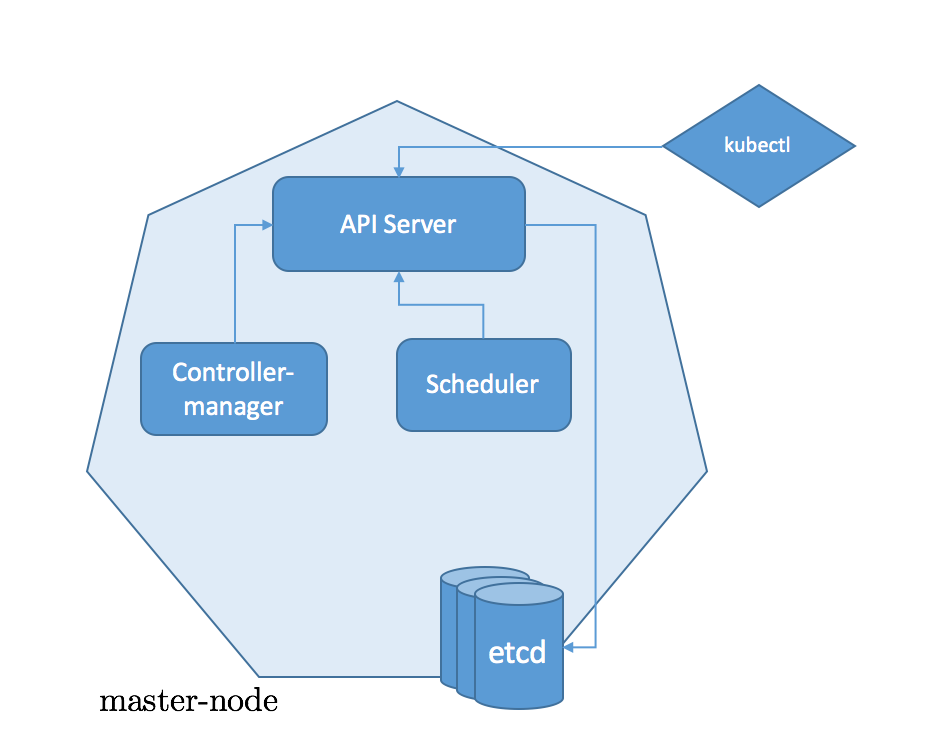
\includegraphics[scale=0.25]{images/img25.png}
\caption{Exemple de master node}
\end{figure}
\end{column}
\begin{column}{0.6\textwidth}
\begin{block}{Master Node}
Le master node est responsable du management du cluster Kubernetes.
\begin{itemize}
\item C'est le point d'entré de toutes les tâches administratives.
\item Il est le responsable de \textit{l'orchestration} des worker-nodes 
\item Il est composé de plusieurs sous éléments.
\end{itemize}
\end{block}
\end{column}
\end{columns}
\begin{block}{Master Node - l'API Server}
\begin{itemize}
\item C'est le point d'entrée pour toutes les commandes utilisé pour contrôler le cluster.
\item Il récupère les commandes (REST), les valides, et les exécutes.  
\item Le résultat de ces commandes est conservé dans \textit{etcd}.
\end{itemize}

\end{block}
\end{frame}


\begin{frame}{Kubernetes Master}

\begin{block}{Master Node - etcd}
\begin{itemize}
\item etcd est utilisé pour partager la configuration et la découverte de service.
\item API pour des opérations CRUD et permet aux nœuds de s'enregistrer %(pour pouvoir être informé d'un changement de configuration)
\end{itemize}
%\vspace{10px}
%Exemple : la création de pod/service, l'état, namespaces, replication information.
\end{block}

\begin{block}{Master Node - kube-scheduler}
Le scheduler permet le deployment de pods configurer et de services sur les nodes.
\begin{itemize}
\item Il possède les informations des ressources disponibles.
\item Il possède également les informations requises pour l'exécution du service.
\item Il choisit l'endroit du déploiement.
\end{itemize}
\end{block}


\begin{block}{Master Node - kube-controller-manager}
C'est un composant qui possède plusieurs controllers.
\begin{itemize}
\item Node Controller : Responsable de la bonne gestion des noeuds.
\item Replication Controller : Responsable du maintient du bon nombre de pods pour chaque ReplicatSet objet du système.
\item Endpoints Controller : Service qui associe service et pods.
\end{itemize}
\end{block}


\end{frame}


\subsection{General Overview}
\begin{frame}{Kubernetes Overview}
\begin{figure}
\centering
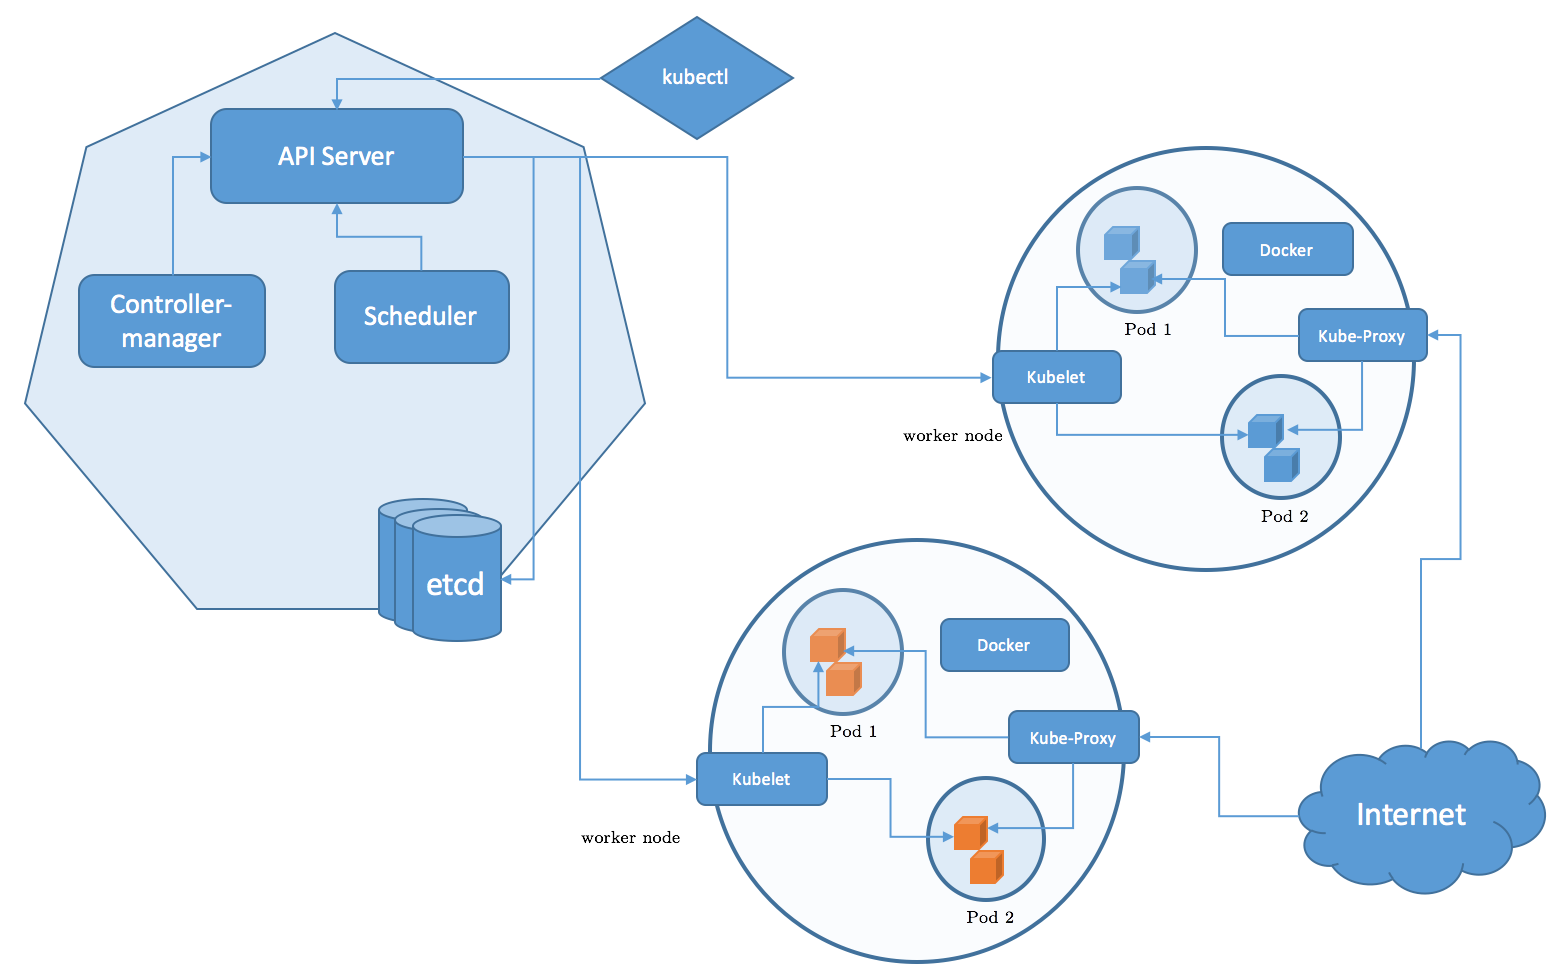
\includegraphics[scale=0.37]{images/img24.png}
\caption{Overview}
\end{figure}
\end{frame}



\section{Kubernetes Scheduler / Replication Controller}
\subsection{Algorithm for the scheduler}
\begin{frame}{Comment Kubernetes Scheduler récupère-t-il un Pod?}
D'après le commit 5871b50 de https://github.com/kubernetes/kubernetes/ il y a 3 grandes étapes : 
\vspace{10px} \\

\textcolor{Framavert}{// Etape 1 : lancement d'une goroutine sched.scheduleOne\\}
\textcolor{Framarouge}{go} wait.\textcolor{Framableu}{Until}(sched.scheduleOne, \textcolor{Framableu}{0}, sched.config.StopEverything) \pause
\vspace{10px}\\
\textcolor{Framarouge}{func }\textcolor{Framaviolet}{(}\textcolor{Framaorange}{sched }\textcolor{Framaviolet}{*}\textcolor{Framaorange}{Scheduler}\textcolor{Framaviolet}{)} \textcolor{Framaviolet}{scheduleOne}() \{ \textcolor{Framavert}{// Etape 2  : Récupération du prochain pod} \\
\hspace{10px}	pod \textcolor{Framarouge}{:=} sched.config.\textcolor{Framableu}{getNextPod}() \\
\hspace{10px}    \textcolor{Framavert}{// Autres élements du scheduler}\\
\} \\ \pause
\vspace{10px}
\textcolor{Framarouge}{func} \textcolor{Framaviolet}{(}
\textcolor{Framaorange}{c} \textcolor{Framaviolet}{*}\textcolor{Framaorange}{configFactory}\textcolor{Framaviolet}{) getNextPod()} *\textcolor{Framaorange}{v1.Pod} \{  \\
\hspace{10px}pod, err \textcolor{Framarouge}{:=} c.podQueue.\textcolor{Framableu}{Pop}() \textcolor{Framavert}{// Etape 3 : On retire le pod d'une file de Pod}\\
\hspace{10px}\textcolor{Framaorange}{if} err == \textcolor{Framableu}{nil} \{ \\
\hspace{10px}\hspace{10px}	return pod \\
\hspace{10px}	\} \\
\hspace{10px}	return  \textcolor{Framableu}{nil}\\
\} \pause
\textcolor{Framavert}{//Les pods sont ajouté à la queue par un EventHandler}

\end{frame}

\begin{frame}{Comment Kubernetes Scheduler détermine-t-il le bon node pour ce pod?}
TODO : \url{https://www.youtube.com/watch?v=bbPcb2JuJPw&t=601s}
\end{frame}

\subsection{Algorithm for the Replication Controller}
\begin{frame}{Mon petit Replication Controller}

\end{frame}


\section{Conclusion}
\subsection{Conclusion}
\begin{frame}{Conclusion}

\end{frame}

\subsection{Références}


\begin{frame}{Références}
\begin{itemize}
\item Kubernetes Documentation. 2018. Nodes | Kubernetes. [ONLINE] Available at: \url{https://kubernetes.io/docs/concepts/architecture/nodes/}. [Accessed 10 February 2018].
\item Kubernetes Documentation. 2018. Service | Kubernetes. [ONLINE] Available at: \url{https://kubernetes.io/docs/concepts/services-networking/service/}. [Accessed 10 February 2018].
\item Kubernetes Documentation. 2018. Pods | Kubernetes. [ONLINE] Available at: \url{https://kubernetes.io/docs/concepts/workloads/pods/pod-overview/}. [Accessed 10 February 2018].
\item Kubernetes Documentation. 2018. Concepts | Kubernetes. [ONLINE] Available at: \url{https://kubernetes.io/docs/concepts/}. [Accessed 10 February 2018].
\item acmqueue, BRENDAN BURNS, BRIAN GRANT, DAVID OPPENHEIMER, ERIC BREWER, AND JOHN WILKES, GOOGLE INC., 2016. Borg, Omega, and Kubernetes. System evolution, [Online]. 14/1, 70. Available at: \url{https://queue.acm.org/detail.cfm?id=2898444} [Accessed 10 February 2018].
\end{itemize}
\end{frame}

\begin{frame}{Références}
\begin{itemize}
\item Quora - Jorg Brown. 2015. What is Borg at Google?. [ONLINE] Available at: \url{https://www.quora.com/What-is-Borg-at-Google}. [Accessed 10 February 2018].
\item The Morning Paper - Adrian Colyer. 2015. Large-scale cluster management at Google with Borg. [ONLINE] Available at: \url{https://blog.acolyer.org/2015/05/07/large-scale-cluster-management-at-google-with-borg/}. [Accessed 10 February 2018].
\item Carla Schroder. 2017. What Makes Up a Kubernetes Cluster?. [ONLINE] Available at: \url{https://www.linux.com/news/learn/chapter/intro-to-kubernetes/2017/4/what-makes-kubernetes-cluster}. [Accessed 10 February 2018].
\item Fabrice Jammes - Cloud Native Computing Fundation. 2017. Kubernetes et les micro-services. [ONLINE] Available at: \url{https://indico.in2p3.fr/event/16962/attachments/46065/57449/Kube_webinaire_RI3_201801.pdf}. [Accessed 10 February 2018].
\end{itemize}
\end{frame}


\begin{frame}{Références}
\begin{itemize}
\item Nune Isabekyan. 2016. Introduction to Kubernetes Architecture</em>. [ONLINE] Available at: \url{https://x-team.com/blog/introduction-kubernetes-architecture/}. [Accessed 10 February 2018].
\item Julia Evans. 2017. A few things I've learned about Kubernetes. [ONLINE] Available at: \url{https://jvns.ca/blog/2017/06/04/learning-about-kubernetes/}. [Accessed 10 February 2018].
\item Julia Evans. 2018. How does the Kubernetes scheduler work?. [ONLINE] Available at: \url{https://jvns.ca/blog/2017/07/27/how-does-the-kubernetes-scheduler-work/}. [Accessed 10 February 2018].
\item YouTube. (2018). Kubernetes Scheduling Features or How Can I Make the System Do What I Want? [I] - Marek Grabowski. [Online Video]. 17 April 2017. Available from: \url{https://www.youtube.com/watch?v=bbPcb2JuJPw&t=601s}. [Accessed: 10 February 2018].
\end{itemize}
\end{frame}


\begin{frame}{Références}
\begin{itemize}

\item YouTube. (2018). Container clusters with Kubernetes -Tim Hockin. [Online Video]. 21 April 2015. Available from: \url{https://www.youtube.com/watch?v=KIdK5WGZUms}. [Accessed: 10 February 2018].
\item YouTube. (2018). Dockers Containers \& Kubernetes - Brian Dorsey. [Online Video]. 7 June 2015. Available from: \url{https://www.youtube.com/watch?v=KIdK5WGZUms}. [Accessed: 10 February 2018].
\end{itemize}
\end{frame}

\end{document}





